\documentclass[12pt,a4paper]{report}

% ---------- Packages ----------
\usepackage[a4paper,margin=1in,headheight=15pt]{geometry}
\usepackage[T1]{fontenc}
\usepackage[utf8]{inputenc}
\usepackage{lmodern}
\usepackage{microtype}
\usepackage{setspace}
\usepackage{graphicx}
\usepackage{float}
\usepackage{booktabs}
\usepackage{longtable}
\usepackage{array}
\usepackage{tabularx}
\usepackage{amsmath,amssymb}
\usepackage{hyperref}
\usepackage{xcolor}
\usepackage{caption}
\usepackage{subcaption}
\usepackage{fancyhdr}
\usepackage{tikz}
\usetikzlibrary{arrows.meta,positioning,shapes.geometric,fit,calc}

\hypersetup{
  colorlinks=true,
  linkcolor=blue!45!black,
  citecolor=blue!45!black,
  urlcolor=blue!55!black,
  pdftitle={FraudShield: AI-Based Financial Transaction Fraud Detection},
  pdfauthor={Muhammad Rafay, Zohaib Tariq, Syed Muhammad Aqib}
}
\setstretch{1.25}
\setlength{\parskip}{5pt}
\setlength{\parindent}{0pt}
\pagestyle{fancy}
\fancyhf{}
\fancyhead[L]{FraudShield}
\fancyhead[R]{AI \& Expert Systems}
\fancyfoot[C]{\thepage}
\renewcommand{\headrulewidth}{0.4pt}

\newcommand{\dataset}[1]{\textit{#1}}
\newcommand{\metric}[1]{\textsc{#1}}

\begin{document}

% ============================================================
% TITLE PAGE
% ============================================================
\begin{titlepage}
  \centering
  \vspace*{0.5cm}
  % University logo placeholder: place NED.png in the same directory.
  \IfFileExists{NED.png}{
    
\includegraphics[width=0.22\textwidth]{NED.png}
  }{
    \fbox{\parbox[c][3.0cm][c]{0.30\textwidth}{\centering University Logo\\[3pt]\texttt{NED.png}}}
  }

  \vspace{1.0cm}
  {\Large\bfseries NED University of Engineering \& Technology\par}
  \vspace{0.25cm}
  {\large Department of Computer Science \& Information Technology\par}
  \vspace{1.0cm}
  {\Large\bfseries CT-361: Artificial Intelligence \& Expert System\par}
  \vspace{0.5cm}
  {\huge\bfseries FraudShield\par}
  \vspace{0.25cm}
  {\LARGE AI-Based Financial Transaction Fraud Detection\par}
  \vspace{0.6cm}
  {\large Complex Computing Problem (CCP) Technical Report\par}

  \vfill
  \begin{tabular}{>{\bfseries}rl}
    Team Members: & Muhammad Rafay (CT-24141)\\
                  & Zohaib Tariq (CT-24149)\\
                  & Syed Muhammad Aqib (CT-24150)\\
  \end{tabular}

  \vfill
  {\large Academic Project Report\par}
  {\large \today\par}
\end{titlepage}

\pagenumbering{roman}
\chapter*{Abstract}
Financial transaction fraud creates direct losses for customers and financial institutions and can weaken trust in digital payment services. This project, named \textbf{FraudShield}, develops a supervised machine-learning pipeline for identifying potentially fraudulent transactions in two distinct settings: mobile-money transfers and card payments. The implementation uses the PaySim mobile-money dataset and the Sparkov simulated card-transaction dataset. A Logistic Regression classifier is used as the baseline, and its performance is compared with Random Forest, XGBoost, and tuned versions of both tree-based models.

The training notebook applies dataset-specific preprocessing, class-imbalance handling, model tuning with stratified cross-validation, validation-based threshold selection, and final evaluation on held-out test data. The model selected for each dataset is the tuned Random Forest. On PaySim, it obtains a test precision of 1.0000, recall of 0.9976, F1-score of 0.9988, and PR-AUC of 0.9982. On Sparkov, it obtains precision of 0.8701, recall of 0.7622, F1-score of 0.8126, and PR-AUC of 0.8598. The results show that a single model family and a single feature representation are not assumed to fit every payment domain; instead, separate specialist models are trained for the two datasets.

The report documents the problem, datasets, preprocessing, model design, experimental protocol, results, limitations, ethical considerations, and future improvements. A methodology flowchart is included as a TikZ diagram so that it can be compiled directly from this LaTeX source.

\textbf{Keywords:} financial fraud detection, PaySim, Sparkov, class imbalance, Random Forest, XGBoost, Logistic Regression, PR-AUC.

\clearpage
\pagenumbering{arabic}

% ============================================================
\chapter{Introduction}
\section{Background}
Digital financial services support large volumes of mobile-money transfers and card payments. The convenience and speed of these systems also create opportunities for fraudulent activity. Fraudulent transactions may resemble legitimate transactions in amount, timing, merchant category, or account activity. Rule-based checks can be useful for known patterns, but fixed rules may not capture complex relationships among transaction attributes.

Machine learning provides a data-driven approach: a model learns patterns from historical examples labelled as fraudulent or legitimate and estimates the probability that a new transaction belongs to the fraud class. In a practical fraud-monitoring system, the probability is converted into an operational decision using a threshold. This threshold matters because false negatives represent missed fraud, while false positives can interrupt legitimate customers and create investigation workload.

\section{Problem statement}
The project addresses the problem of identifying fraudulent financial transactions from structured transaction data. The real-world impact includes monetary loss, customer inconvenience, operational cost, and reduced confidence in digital payment platforms. Fraud is typically a minority class, so a model that simply predicts the majority class can achieve apparently strong accuracy while detecting very little fraud.

FraudShield applies supervised classification to two transaction domains. It trains a dedicated model for mobile-money transactions and another for card transactions. The models output fraud probabilities and use validation-selected decision thresholds to classify transactions as legitimate or potentially fraudulent.

\section{Project objectives}
The main objectives are:
\begin{enumerate}
  \item Use at least two relevant datasets representing different financial transaction settings.
  \item Prepare the datasets using domain-aware feature selection and preprocessing.
  \item Establish Logistic Regression as a baseline and compare it with Random Forest and XGBoost.
  \item Tune the tree-based models using randomized hyperparameter search and PR-AUC.
  \item Select models using validation data, tune decision thresholds using validation F1, and evaluate once on held-out test data.
  \item Report performance using precision, recall, F1-score, ROC-AUC, and PR-AUC.
  \item Consider privacy, transparency, and operational limitations.
\end{enumerate}

\section{Scope}
The project includes both an offline training workflow and a working monitoring prototype. The notebooks load prepared CSV files, train and evaluate the specialist models, and save model artifacts and metadata. A FastAPI backend loads those artifacts and exposes health, prediction, persistent transaction, analytics, model-information, and server-sent event endpoints. A React dashboard consumes these endpoints to provide channel filtering, risk charts, a recent-transaction feed, model-performance summaries, manual transaction analysis, and illustrative live traffic simulation. This is a functional prototype rather than a production payment gateway: authentication, deployment hardening, automated retraining, and human case management remain outside the current scope.

% ============================================================
\chapter{Datasets and Data Understanding}
\section{Dataset sources}
Two datasets are used, satisfying the CCP requirement for at least two relevant data sources.

\begin{table}[H]
\centering
\caption{Datasets used in FraudShield}
\begin{tabularx}{\textwidth}{p{2.5cm}p{3.0cm}X}
\toprule
\textbf{Dataset} & \textbf{Domain and files} & \textbf{Source and relevance}\\
\midrule
PaySim & Mobile-money transactions & Kaggle dataset by ealaxi. It contains transaction types, amounts, account balances, and the \texttt{isFraud} label. It is used to learn patterns associated with fraudulent mobile-money activity.\\
Sparkov & Card transactions & Kaggle dataset by kartik2112. It contains transaction time, category, amount, customer and merchant location fields, demographic fields, and the \texttt{is\_fraud} label. It is used to model card-payment fraud.\\
\bottomrule
\end{tabularx}
\end{table}

\textbf{PaySim source:} \url{https://www.kaggle.com/datasets/ealaxi/paysim1}

\textbf{Sparkov source:} \url{https://www.kaggle.com/datasets/kartik2112/fraud-detection}

The dataset names, fields, and file expectations above follow the supplied training notebook. The Kaggle pages are the originating distribution pages provided for this project.

\section{PaySim characteristics and preparation}
The notebook loads 6,362,620 rows and 11 columns. It reports no missing values and a fraud rate of 0.1291\%. The target is \texttt{isFraud}. The notebook derives two balance consistency features:
\[
\texttt{errorBalanceOrig} =
\texttt{newbalanceOrig}+\texttt{amount}-\texttt{oldbalanceOrg}
\]
\[
\texttt{errorBalanceDest} =
\texttt{oldbalanceDest}+\texttt{amount}-\texttt{newbalanceDest}.
\]
The categorical input is \texttt{type}. Numeric inputs are \texttt{amount}, \texttt{oldbalanceOrg}, \texttt{newbalanceOrig}, \texttt{oldbalanceDest}, \texttt{newbalanceDest}, and the two derived balance-error features. The notebook drops \texttt{nameOrig}, \texttt{nameDest}, \texttt{step}, and \texttt{isFlaggedFraud} from the model feature set. The label is retained separately as the target.

A stratified 80/20 split first creates a development portion and a test portion. The development portion is then split 80/20 into fitting and validation subsets. This results in approximately 64\% fitting data, 16\% validation data, and 20\% held-out test data. The fixed random seed is 42.

\section{Sparkov characteristics and preparation}
The notebook loads 1,296,675 rows from \texttt{fraudTrain.csv} and 555,719 rows from \texttt{fraudTest.csv}. It reports no missing values and a fraud rate of 0.5789\% in the training file. The dataset's provided train and test files are preserved as separate partitions. The training file is sorted by transaction timestamp; its most recent 20\% is used for validation, while the earlier 80\% is used for fitting. The separate test file is treated as the later-period test set.

The notebook does not use customer names, card numbers, street addresses, job titles, or merchant names as model inputs. It engineers the following features:
\begin{itemize}
  \item \texttt{category}: transaction category (categorical);
  \item \texttt{amt}: transaction amount;
  \item \texttt{city\_pop}: population of the customer's city;
  \item \texttt{hour}: hour of day extracted from the transaction timestamp;
  \item \texttt{day\_of\_week}: weekday extracted from the timestamp;
  \item \texttt{age}: age in years, estimated from transaction date and date of birth;
  \item \texttt{distance\_km}: distance between customer and merchant coordinates, computed with the Haversine formula.
\end{itemize}
The model uses \texttt{category} as the categorical feature and the remaining six fields as numeric features.

% ============================================================
\chapter{Methodology}
\section{Overall approach}
FraudShield follows a repeatable pipeline for each dataset. The two datasets are not concatenated into one training table because they represent different transaction domains and have different schemas. Instead, the same experimental protocol is applied independently, producing two specialist models.

\section{Methodology flowchart}
Figure~\ref{fig:methodology} summarizes the implemented workflow. The diagram is authored in TikZ and is therefore part of this source file; no external methodology image is required.

\begin{figure}[H]
\centering
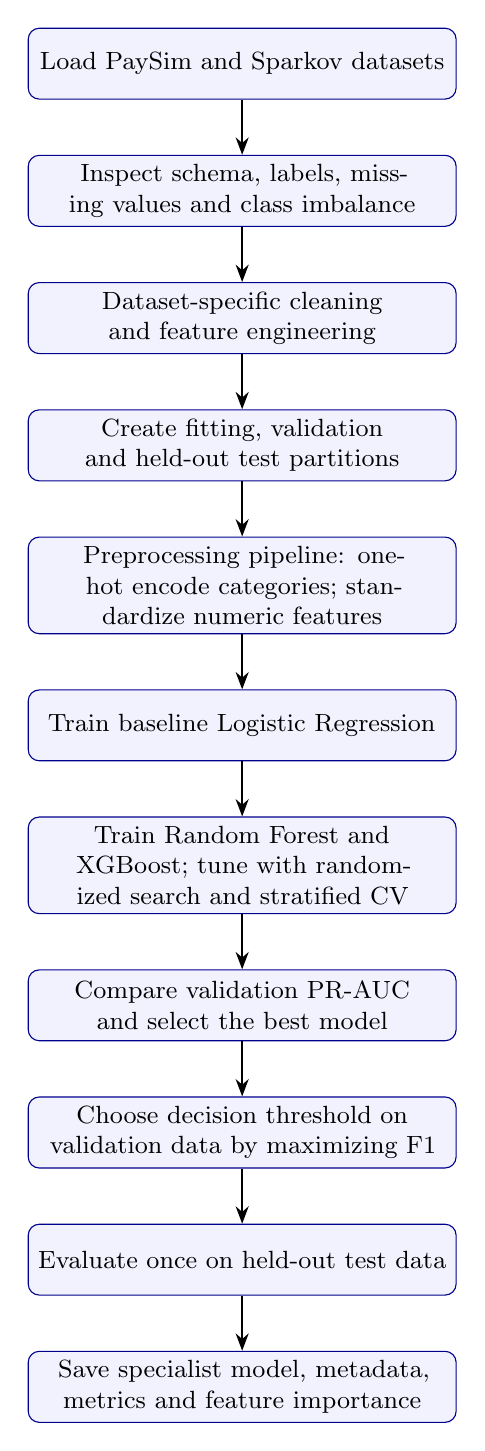
\begin{tikzpicture}[
  node distance=7mm and 12mm,
  process/.style={rectangle, rounded corners, draw=blue!55!black, fill=blue!5,
                  text width=5.2cm, minimum height=9mm, align=center, font=\small},
  decision/.style={diamond, aspect=2.3, draw=orange!70!black, fill=orange!8,
                   text width=2.8cm, align=center, font=\small, inner sep=1pt},
  arrow/.style={-{Stealth[length=2.2mm]}, thick}
]
\node[process] (data) {Load PaySim and Sparkov datasets};
\node[process, below=of data] (inspect) {Inspect schema, labels, missing values and class imbalance};
\node[process, below=of inspect] (prep) {Dataset-specific cleaning and feature engineering};
\node[process, below=of prep] (split) {Create fitting, validation and held-out test partitions};
\node[process, below=of split] (encode) {Preprocessing pipeline: one-hot encode categories; standardize numeric features};
\node[process, below=of encode] (baseline) {Train baseline Logistic Regression};
\node[process, below=of baseline] (models) {Train Random Forest and XGBoost; tune with randomized search and stratified CV};
\node[process, below=of models] (validate) {Compare validation PR-AUC and select the best model};
\node[process, below=of validate] (threshold) {Choose decision threshold on validation data by maximizing F1};
\node[process, below=of threshold] (test) {Evaluate once on held-out test data};
\node[process, below=of test] (save) {Save specialist model, metadata, metrics and feature importance};
\draw[arrow] (data) -- (inspect);
\draw[arrow] (inspect) -- (prep);
\draw[arrow] (prep) -- (split);
\draw[arrow] (split) -- (encode);
\draw[arrow] (encode) -- (baseline);
\draw[arrow] (baseline) -- (models);
\draw[arrow] (models) -- (validate);
\draw[arrow] (validate) -- (threshold);
\draw[arrow] (threshold) -- (test);
\draw[arrow] (test) -- (save);
\end{tikzpicture}
\caption{FraudShield methodology implemented in the training notebook. The sequence is run independently for PaySim and Sparkov.}
\label{fig:methodology}
\end{figure}

\section{Preprocessing pipeline}
Categorical features are transformed using \texttt{OneHotEncoder(handle\_unknown="ignore")}. Numeric features are transformed using \texttt{StandardScaler}. Both operations are combined with a \texttt{ColumnTransformer} inside a scikit-learn \texttt{Pipeline}. Keeping preprocessing inside the pipeline ensures that the transformations are fitted on the fitting partition and then applied consistently to validation and test data.

The implementation uses class imbalance controls. Logistic Regression uses \texttt{class\_weight="balanced"}, Random Forest uses \texttt{class\_weight="balanced\_subsample"}, and XGBoost uses \texttt{scale\_pos\_weight}, calculated from the negative-to-positive class ratio in the fitting data.

\section{Models}
\subsection{Logistic Regression baseline}
Logistic Regression is the baseline classifier. It uses balanced class weights and a maximum of 1,000 iterations. It provides a comparatively simple reference point against which the more flexible tree-based classifiers can be evaluated.

\subsection{Random Forest}
The initial Random Forest uses 100 trees, maximum depth 12, balanced subsampling, all available CPU cores, and random seed 42. The tuned search space includes the number of estimators, maximum depth, minimum samples per leaf, and maximum features considered at a split.

\subsection{XGBoost}
The initial XGBoost model uses 300 estimators, maximum depth 6, learning rate 0.1, histogram-based tree construction, and PR-AUC-oriented evaluation. Its positive-class weight is set using the class ratio. The tuning search varies the number of estimators, depth, learning rate, row subsampling, column subsampling, and minimum child weight.

\section{Hyperparameter tuning}
Randomized search is used for Random Forest and XGBoost. The notebook evaluates six parameter combinations per model (\texttt{N\_ITER=6}) using three-fold stratified cross-validation. The search scoring metric is average precision, which corresponds to PR-AUC in the notebook. If the fitting partition exceeds 300,000 rows, a stratified sample of 300,000 rows is used for the search; the selected configuration is subsequently fitted on the full fitting partition.

\section{Model selection and threshold selection}
The model-selection rule is the highest validation PR-AUC. The test set is not used to select the model. For each candidate model, the decision threshold is selected from the validation precision-recall curve by maximizing F1-score. The chosen threshold is then applied to test probabilities to compute precision, recall, and F1. This separates ranking quality (PR-AUC) from the operating point (threshold-dependent metrics).

\section{Evaluation metrics}
\begin{itemize}
  \item \textbf{Precision:} fraction of transactions flagged as fraud that are actually fraud.
  \item \textbf{Recall:} fraction of actual fraudulent transactions that are detected.
  \item \textbf{F1-score:} harmonic mean of precision and recall.
  \item \textbf{ROC-AUC:} area under the receiver operating characteristic curve.
  \item \textbf{PR-AUC:} average precision, summarizing the precision-recall curve.
\end{itemize}
PR-AUC is emphasized because fraud is rare in both datasets. Under severe class imbalance, ROC-AUC can remain high even when the precision of fraud alerts is comparatively weak.

% ============================================================
\chapter{Experimental Setup}
\section{Reproducibility}
The training notebook sets the random seed to 42 for data splitting, randomized search, and model configuration where supported. The principal libraries include pandas, NumPy, scikit-learn, XGBoost, joblib, and Matplotlib. The exact installed library versions are environment-dependent; the notebook records the scikit-learn version in each model metadata file.

\section{Partition sizes}
\begin{table}[H]
\centering
\caption{Partition sizes reported by the training notebook}
\begin{tabular}{lrrr}
\toprule
\textbf{Dataset} & \textbf{Fit} & \textbf{Validation} & \textbf{Test}\\
\midrule
PaySim & 4,072,076 & 1,018,020 & 1,272,524\\
Sparkov & 1,037,340 & 259,335 & 555,719\\
\bottomrule
\end{tabular}
\end{table}

For PaySim, the partitions are created by stratified random splitting. For Sparkov, the training file is ordered by time and the last 20\% is reserved for validation; the separate supplied test file is evaluated afterward. The two strategies reflect the data organization provided for each source and should be kept in mind when interpreting cross-dataset comparisons.

\section{Selected model configurations}
The best Random Forest search configuration reported for PaySim is 300 estimators, maximum depth 20, minimum leaf size 5, and \texttt{sqrt} maximum features. The best XGBoost configuration reported for PaySim uses 500 estimators, depth 4, learning rate 0.05, subsample 0.85, column subsample 0.7, and minimum child weight 5.

For Sparkov, the best Random Forest configuration is also 300 estimators, maximum depth 20, minimum leaf size 5, and \texttt{sqrt} maximum features. The best XGBoost configuration uses 300 estimators, depth 6, learning rate 0.1, full row and column subsampling, and minimum child weight 5. The tuned Random Forest is selected as the final model for both datasets based on validation PR-AUC.

% ============================================================
\chapter{Results and Discussion}
\section{Overall model comparison}
Table~\ref{tab:results} reproduces the test metrics reported by the plotting notebook. The star identifies the model selected for each dataset. Threshold-dependent precision, recall, and F1 are measured at the threshold selected using validation data.

\begin{table}[H]
\centering
\caption{Test-set performance for all evaluated models}
\label{tab:results}
\small
\begin{tabular}{llrrrrr}
\toprule
\textbf{Dataset} & \textbf{Model} & \textbf{Prec.} & \textbf{Recall} & \textbf{F1} & \textbf{ROC-AUC} & \textbf{PR-AUC}\\
\midrule
PaySim & Logistic Regression & 0.7607 & 0.4644 & 0.5767 & 0.9900 & 0.5615\\
PaySim & Random Forest & 1.0000 & 0.9939 & 0.9969 & 0.9995 & 0.9987\\
PaySim & XGBoost & 0.9879 & 0.9915 & 0.9897 & 0.9996 & 0.9973\\
PaySim & Random Forest (tuned)$^\star$ & 1.0000 & 0.9976 & 0.9988 & 0.9995 & 0.9982\\
PaySim & XGBoost (tuned) & 0.9855 & 0.9957 & 0.9906 & 0.9996 & 0.9976\\
\midrule
Sparkov & Logistic Regression & 0.1691 & 0.6793 & 0.2708 & 0.9056 & 0.1178\\
Sparkov & Random Forest & 0.8074 & 0.7347 & 0.7693 & 0.9942 & 0.8110\\
Sparkov & XGBoost & 0.8338 & 0.7646 & 0.7977 & 0.9964 & 0.8509\\
Sparkov & Random Forest (tuned)$^\star$ & 0.8701 & 0.7622 & 0.8126 & 0.9967 & 0.8598\\
Sparkov & XGBoost (tuned) & 0.8310 & 0.7590 & 0.7934 & 0.9965 & 0.8542\\
\bottomrule
\end{tabular}
\end{table}

\section{Precision, recall and F1}
Figure~\ref{fig:1} compares precision, recall, and F1 for the five models on each dataset. On PaySim, the tuned Random Forest achieves near-perfect precision and recall at the selected threshold. On Sparkov, the same model family gives the strongest F1 and precision among the evaluated models, although recall is lower than the PaySim result. This difference indicates that the two datasets present different classification difficulty and transaction patterns.

\begin{figure}[H]
\centering
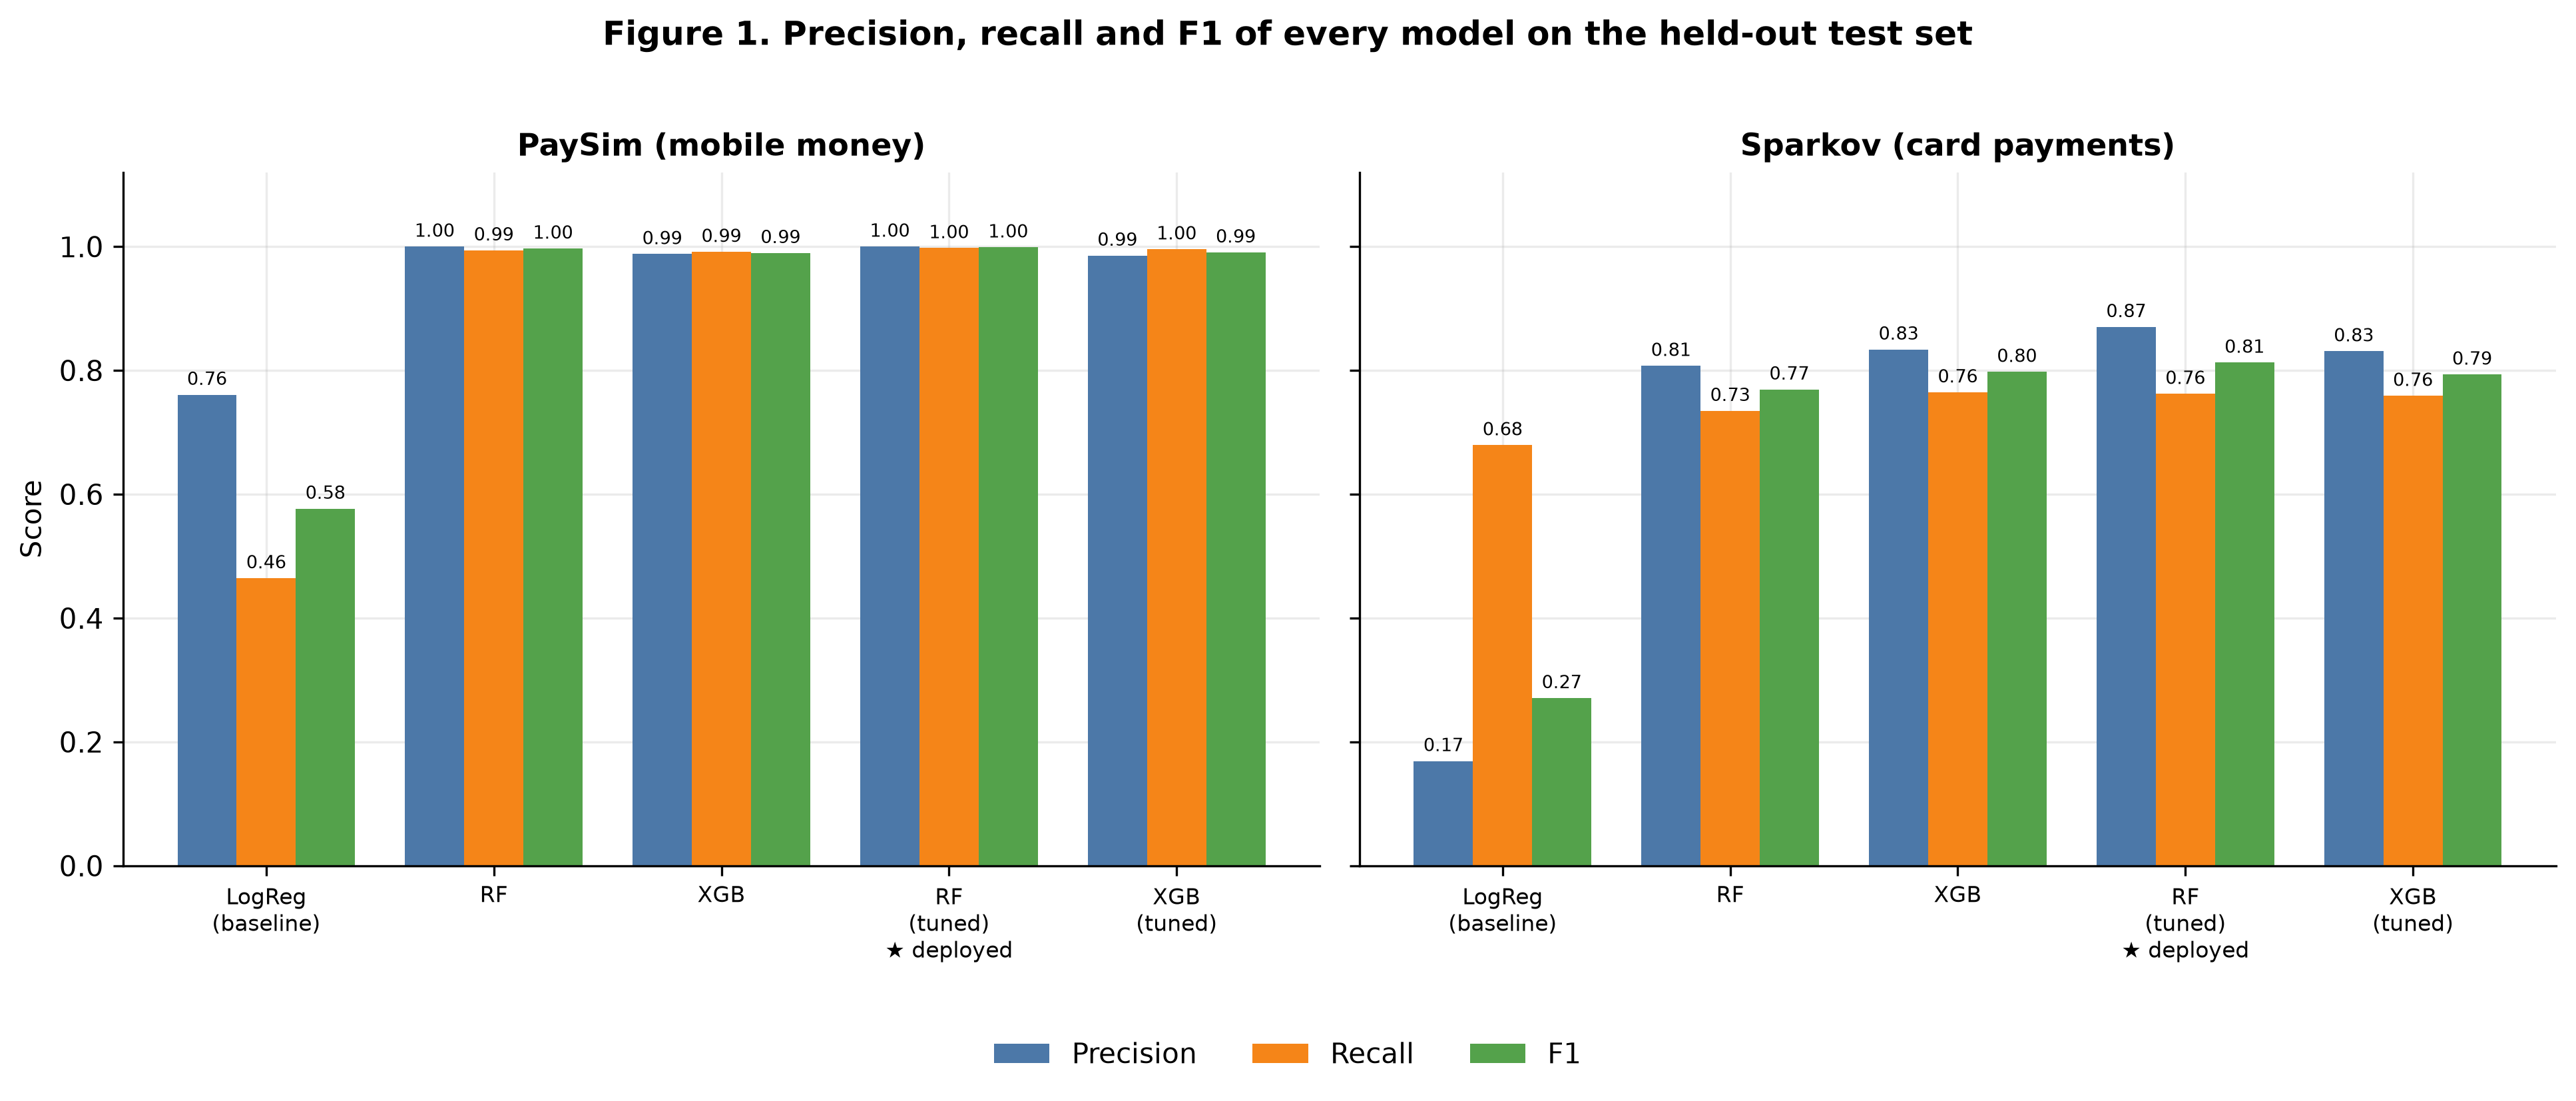
\includegraphics[width=\textwidth]{../reports/figures/fig1.png}
\caption{Precision, recall and F1 of the evaluated models on the held-out test sets.}
\label{fig:1}
\end{figure}

\section{Validation versus test PR-AUC}
Figure~\ref{fig:2} compares validation PR-AUC, used for model selection, with test PR-AUC, reported for final evaluation. PaySim's tuned Random Forest has validation PR-AUC 1.0000 and test PR-AUC 0.9982. Sparkov's tuned Random Forest has validation PR-AUC 0.9040 and test PR-AUC 0.8598. The gap on Sparkov is larger than on PaySim, which suggests that performance on the later-period test data is more challenging than on the validation segment. The test set remains separate from model selection.

\begin{figure}[H]
\centering
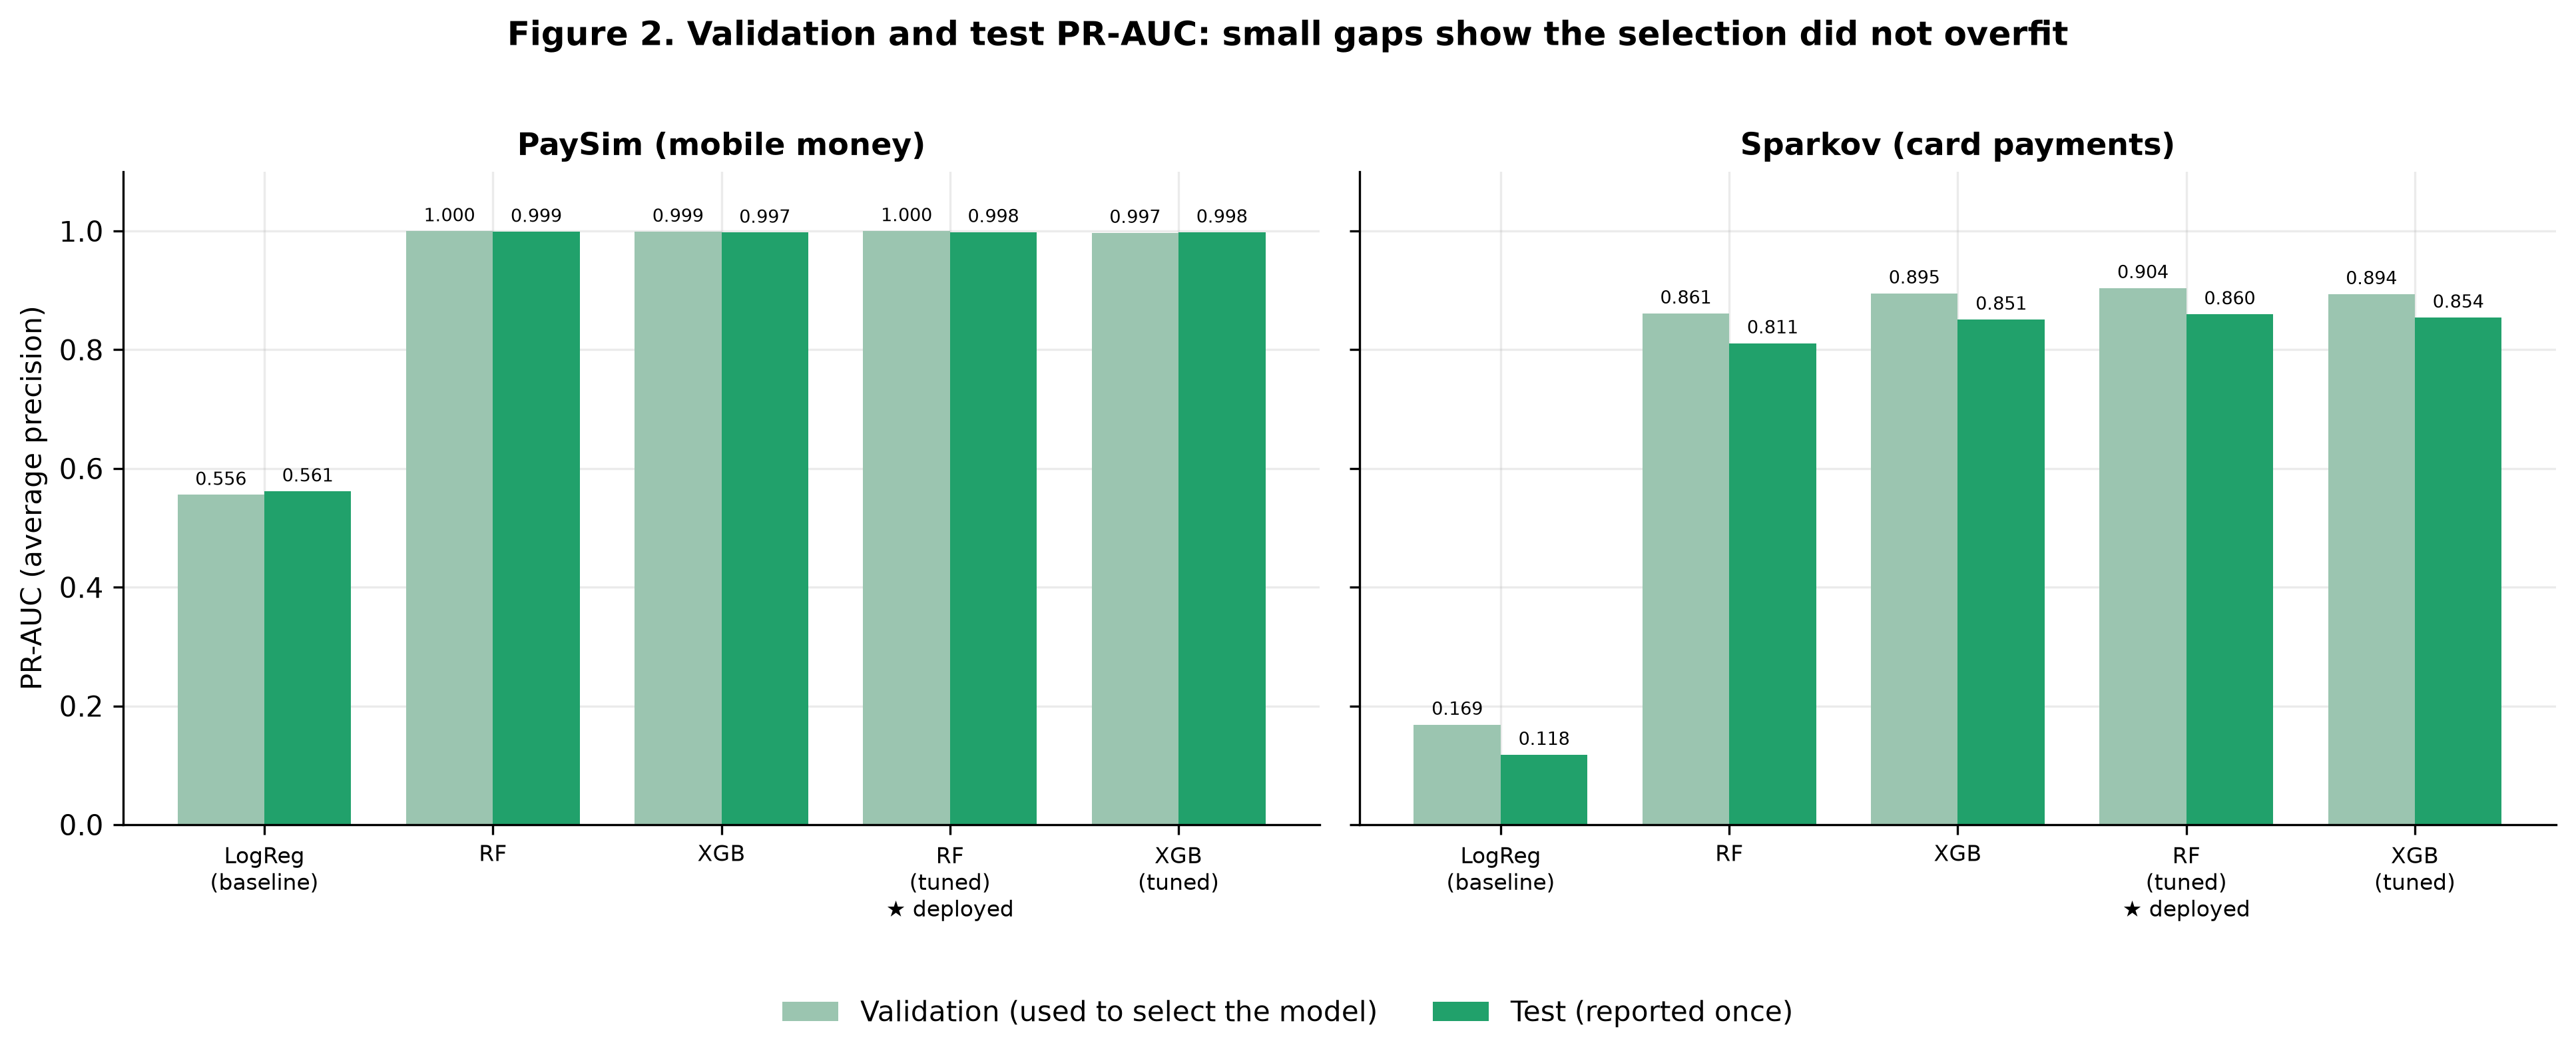
\includegraphics[width=\textwidth]{../reports/figures/fig2.png}
\caption{Validation and test PR-AUC for all candidate models.}
\label{fig:2}
\end{figure}

\section{Effect of decision-threshold tuning}
Figure~\ref{fig:3} compares F1 at the default threshold of 0.5 with F1 at the threshold selected on validation data. The implementation chooses the threshold that maximizes validation F1 for each model. This is important because a probability threshold of 0.5 is not necessarily appropriate when the positive class is rare and training uses class weighting. Threshold tuning provides an operating point that better balances precision and recall for the validation distribution.

\begin{figure}[H]
\centering
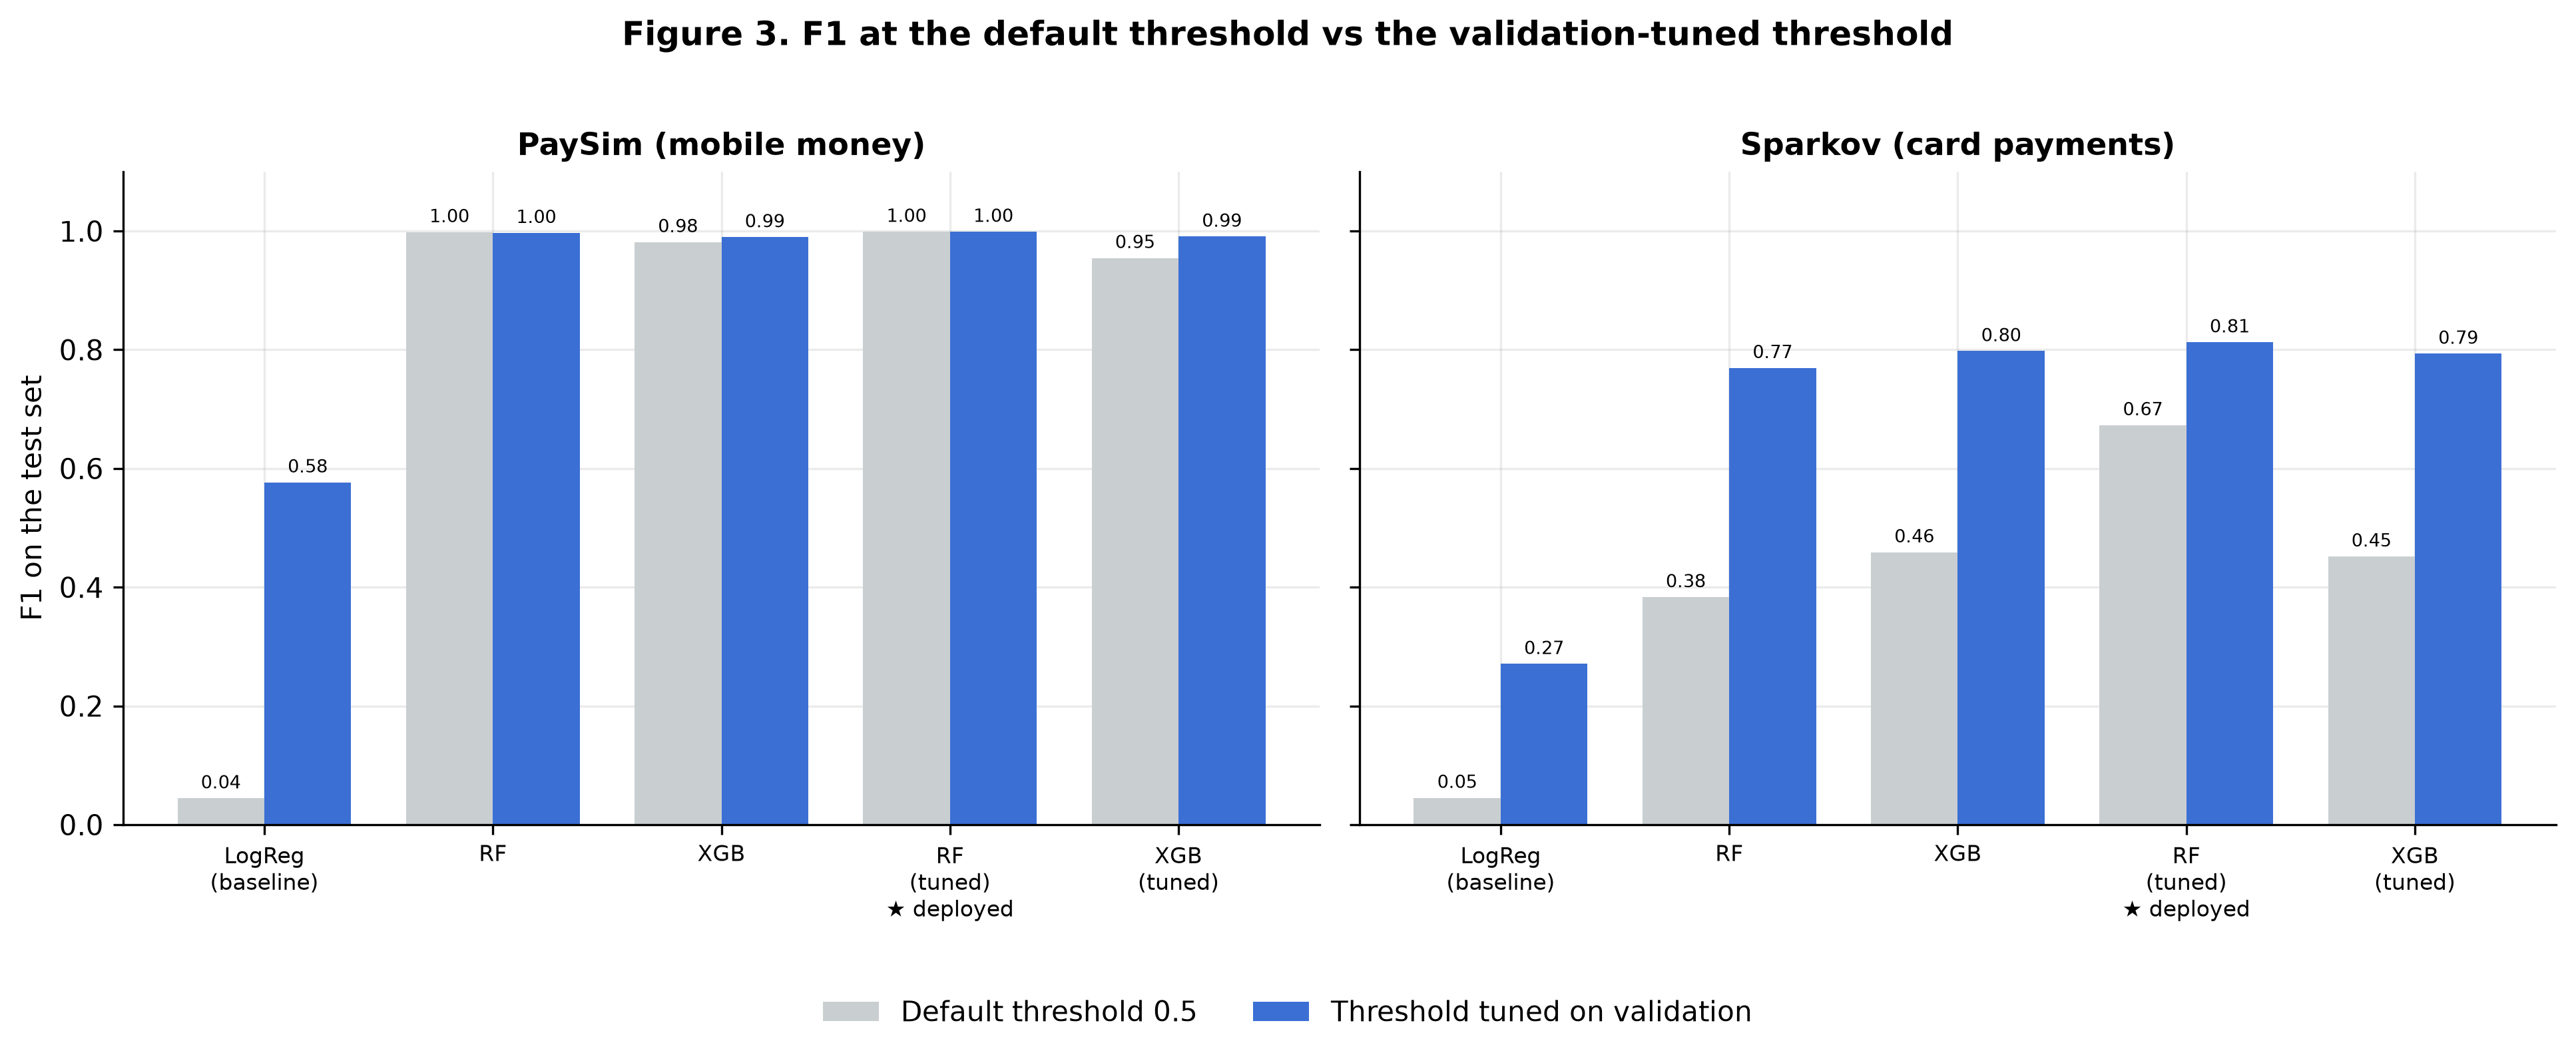
\includegraphics[width=\textwidth]{../reports/figures/fig3.png}
\caption{F1 at the default 0.5 threshold and at the validation-selected threshold.}
\label{fig:3}
\end{figure}

\section{Confusion matrices of the selected models}
The selected PaySim model uses threshold 0.7394 and produces 1,639 true positives, zero false positives, four false negatives, and 1,270,881 true negatives on its test set. The selected Sparkov model uses threshold 0.7749 and produces 1,635 true positives, 244 false positives, 510 false negatives, and 553,330 true negatives. These counts illustrate the different error profiles. A missed fraud is a false negative; a legitimate transaction incorrectly flagged is a false positive.

\begin{figure}[H]
\centering
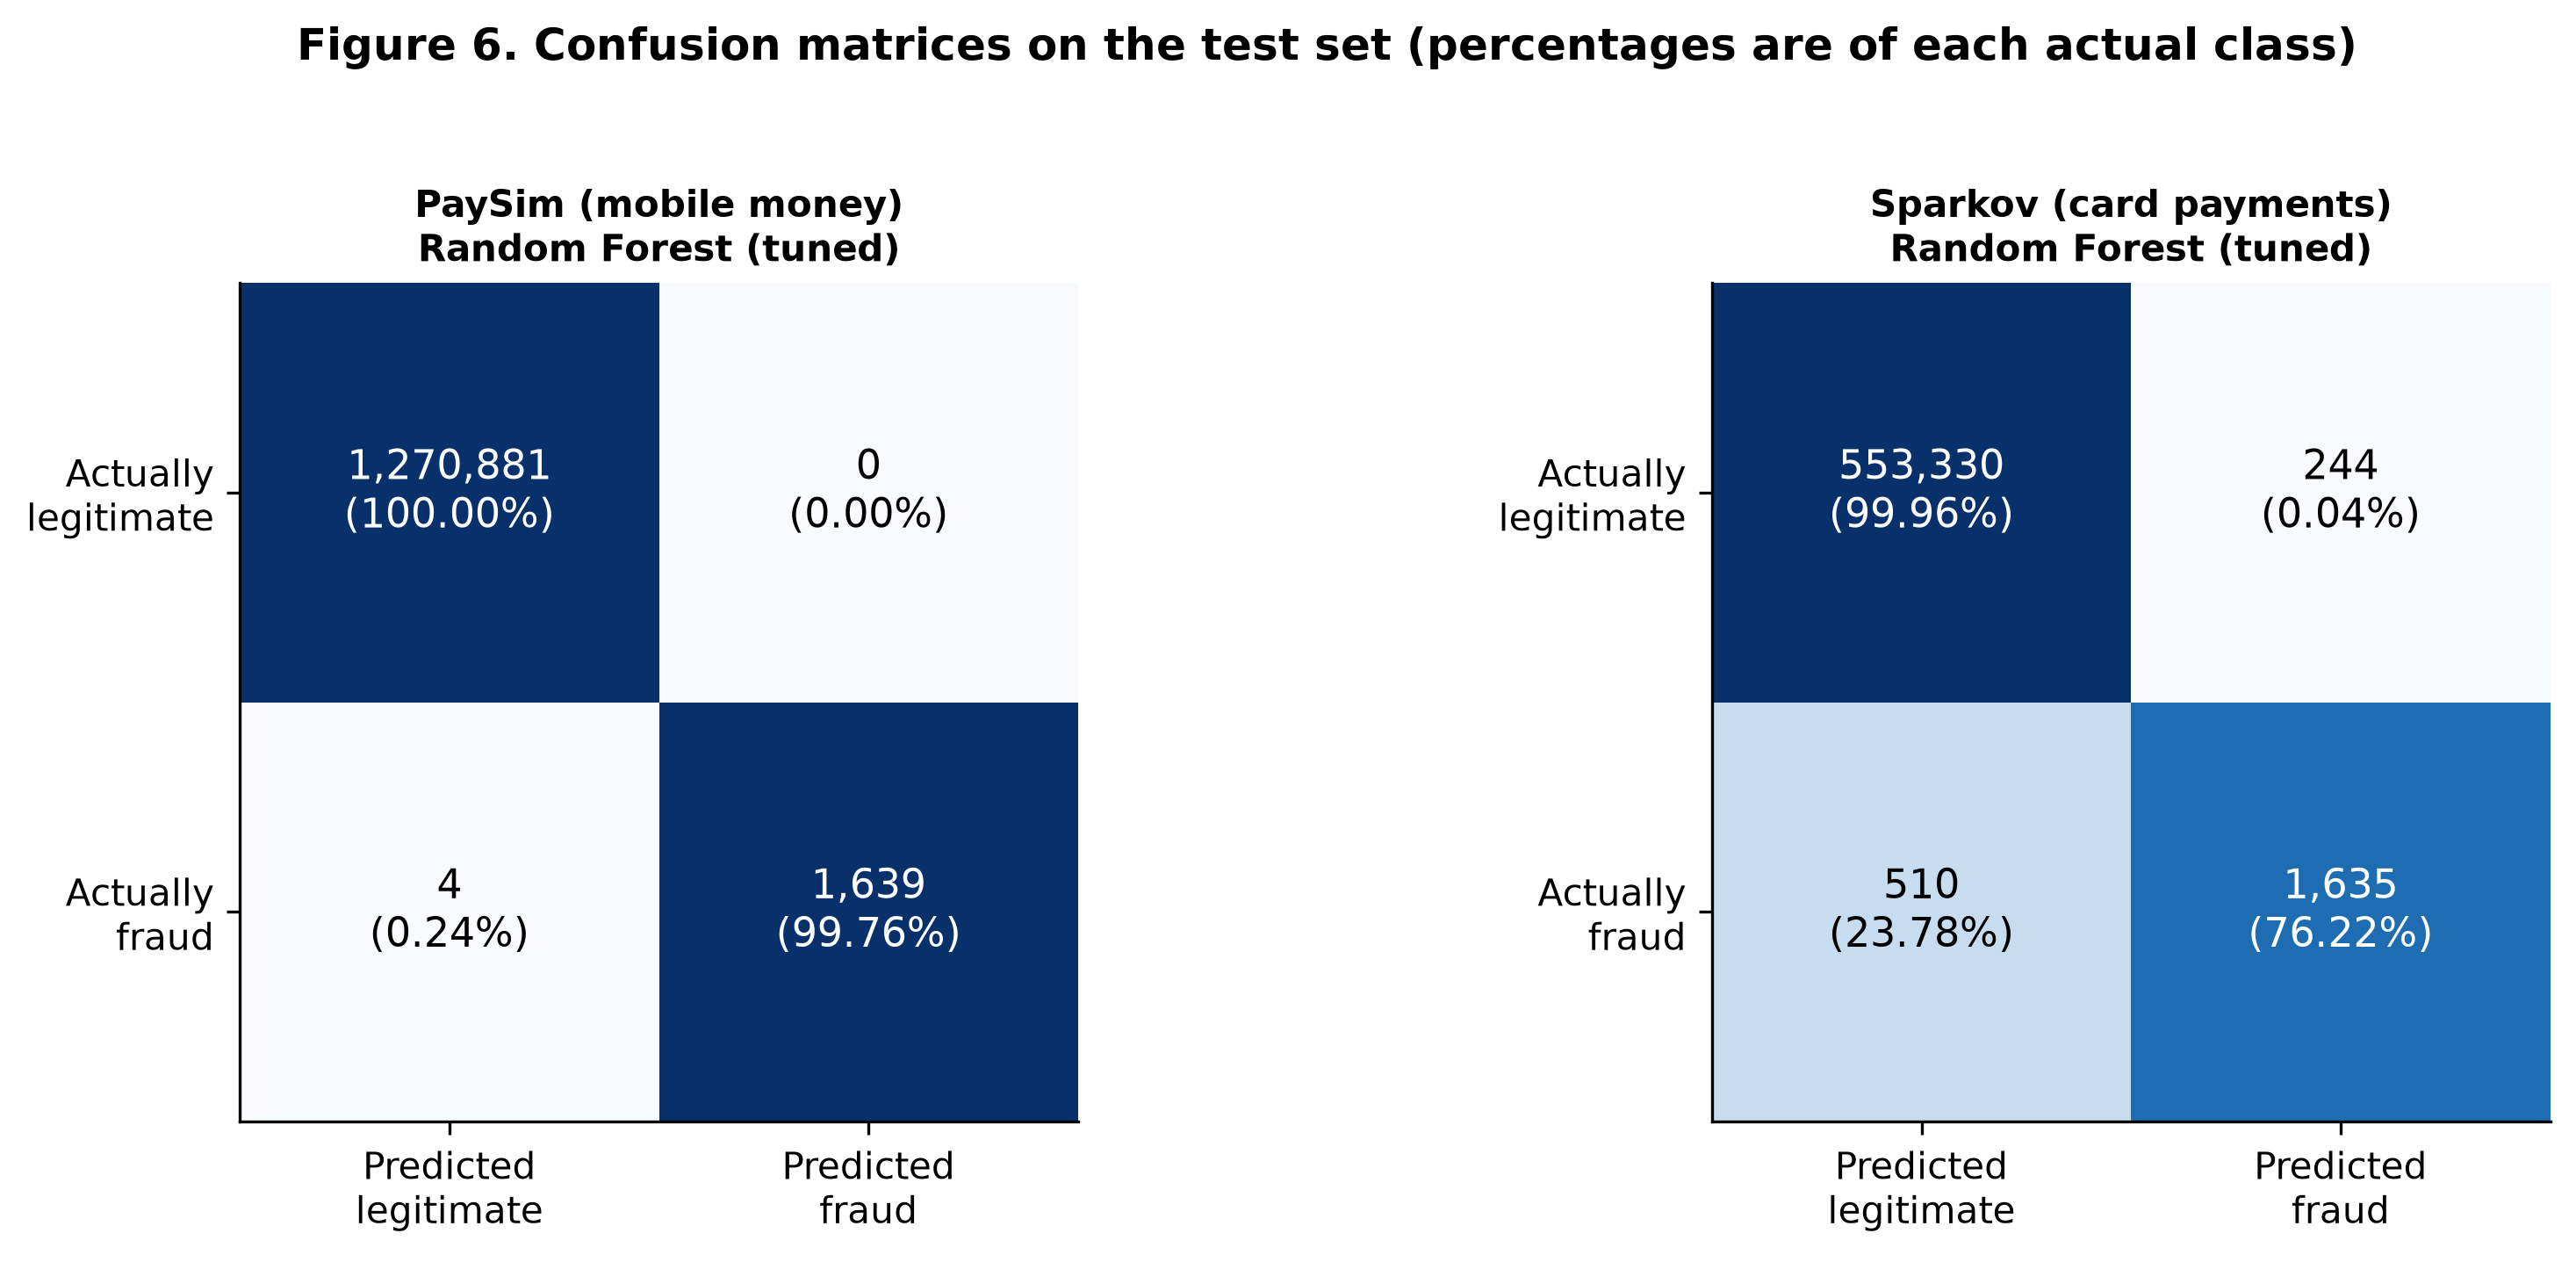
\includegraphics[width=\textwidth]{../reports/figures/fig6.png}
\caption{Confusion matrices for the deployed specialist models on the test sets.}
\label{fig:6}
\end{figure}

\section{Feature importance}
Figure~\ref{fig:7} displays the top eight features reported by each selected model. The notebook obtains tree-model importance from the model's \texttt{feature\_importances\_} attribute. These values indicate which features contribute most to the fitted model's aggregate decisions. They should not be interpreted as causal effects or as a complete explanation for an individual alert. The importance values are comparable within each dataset panel, not necessarily across different model types or datasets.

\begin{figure}[H]
\centering
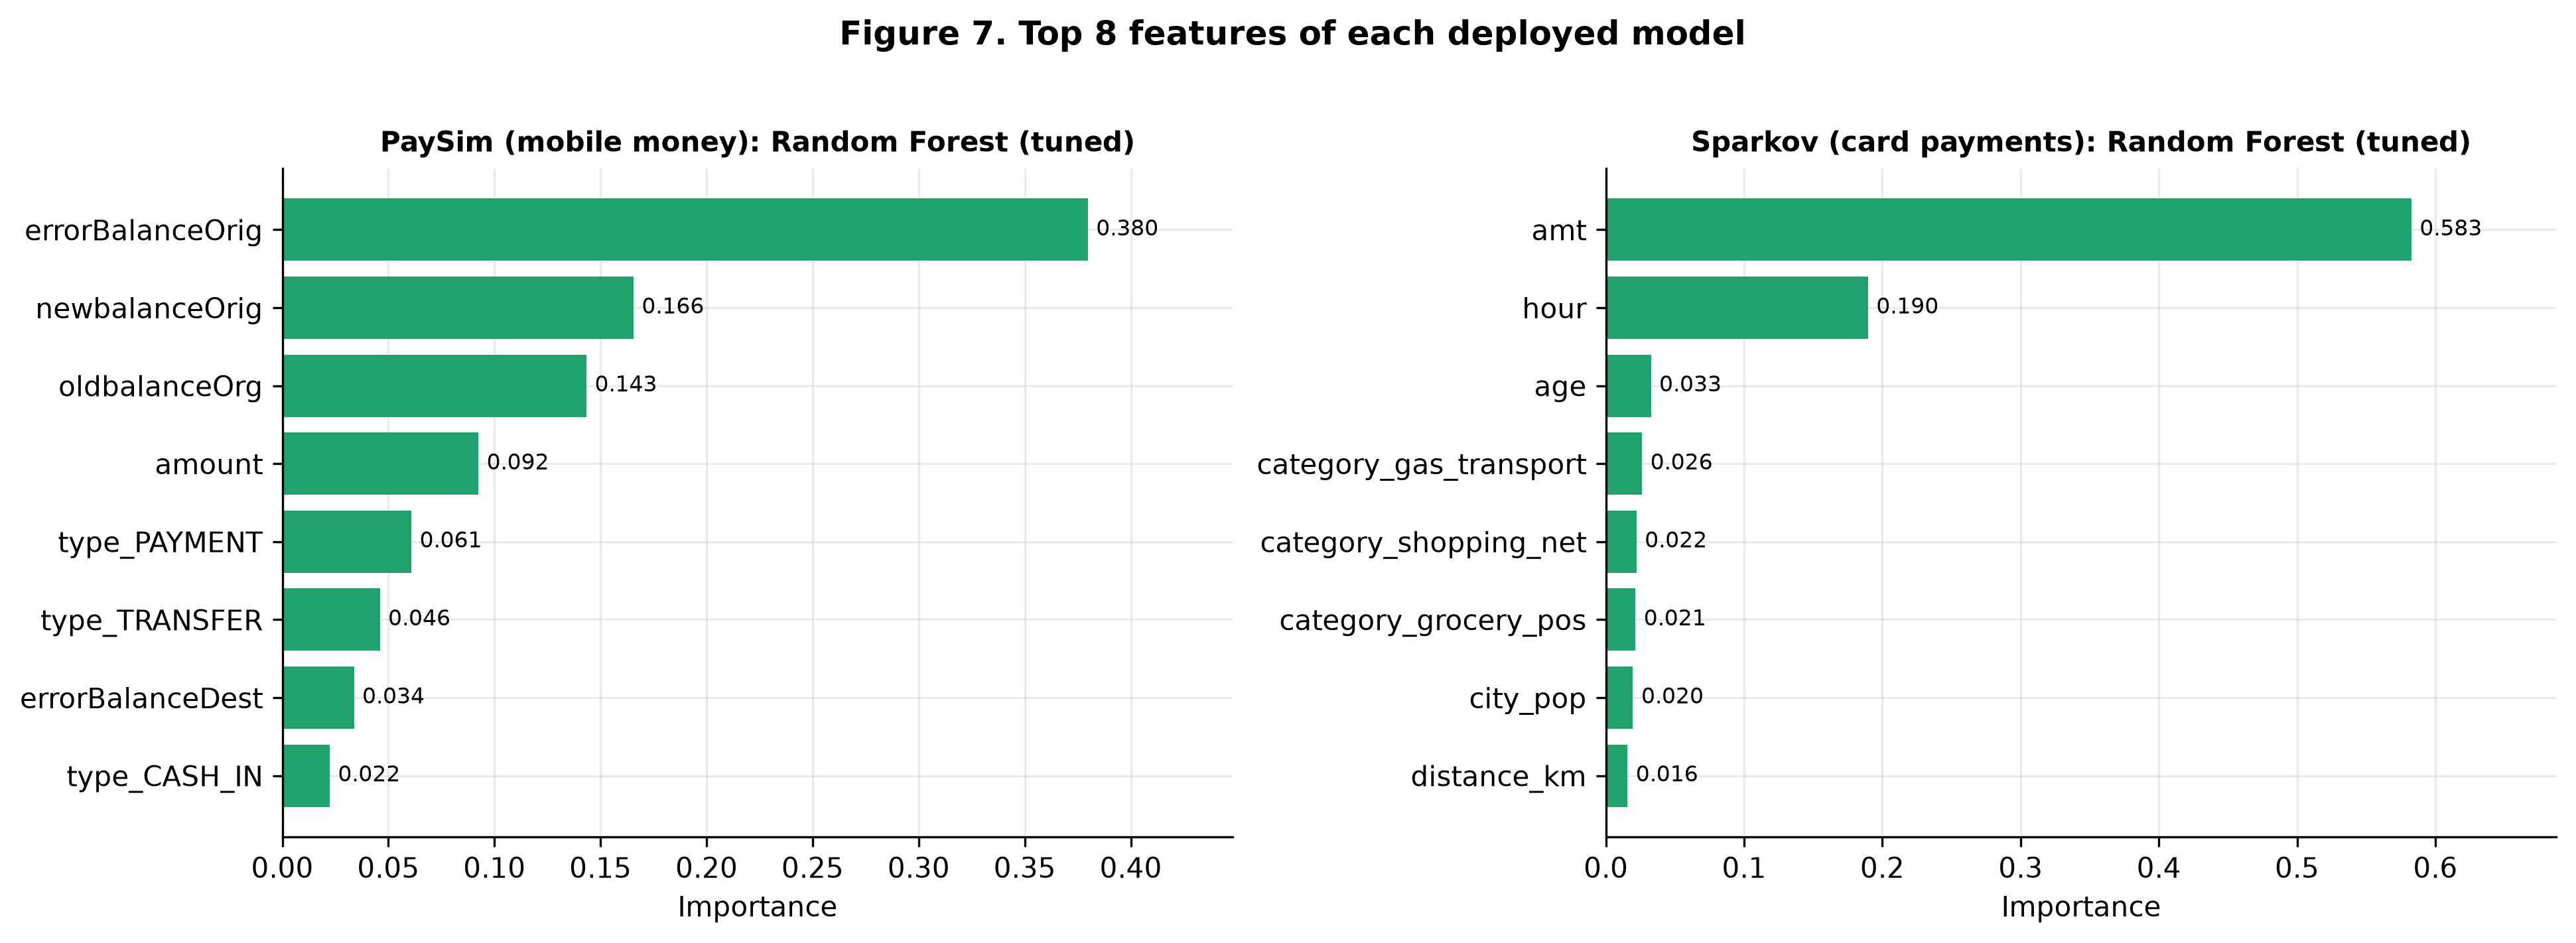
\includegraphics[width=\textwidth]{../reports/figures/fig7.png}
\caption{Top eight feature-importance values for the selected PaySim and Sparkov models.}
\label{fig:7}
\end{figure}

\section{Combined metric view}
Figure~\ref{fig:9} summarizes validation PR-AUC, thresholded precision, recall and F1, ROC-AUC, and test PR-AUC for every model. It reinforces why PR-AUC is important in this task: ROC-AUC values are high for most tree-based models, while PR-AUC more clearly separates the baseline from the stronger classifiers, particularly on Sparkov.

\begin{figure}[H]
\centering
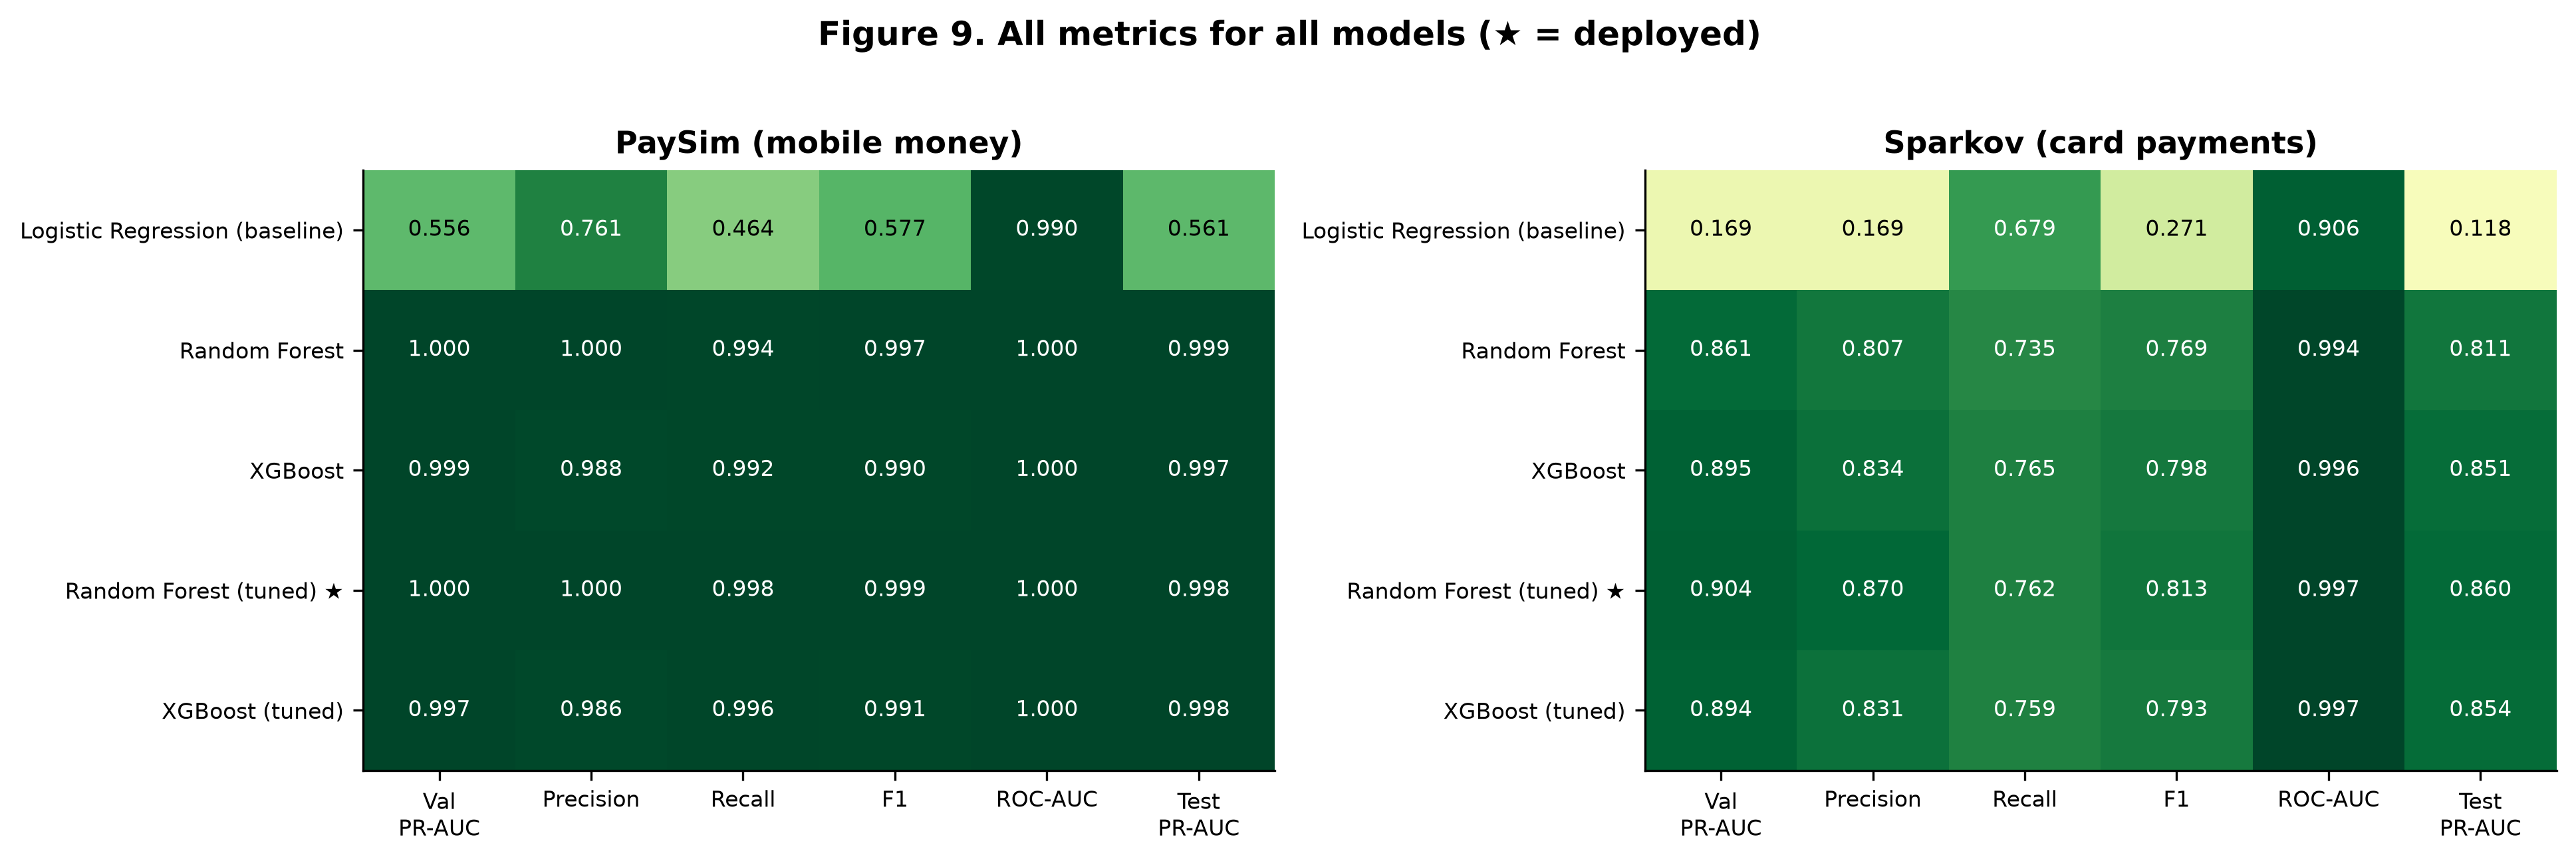
\includegraphics[width=\textwidth]{../reports/figures/fig9.png}
\caption{Heatmap of validation and test metrics for all evaluated models.}
\label{fig:9}
\end{figure}

\section{Precision-recall curves}
Figure~\ref{fig:10} presents the full precision-recall curves generated during training. The curves show performance across possible thresholds, whereas the thresholded metrics in Table~\ref{tab:results} report a single selected operating point. A curve that remains higher over a broad recall range indicates better ranking of fraudulent transactions above legitimate ones.

\begin{figure}[H]
\centering
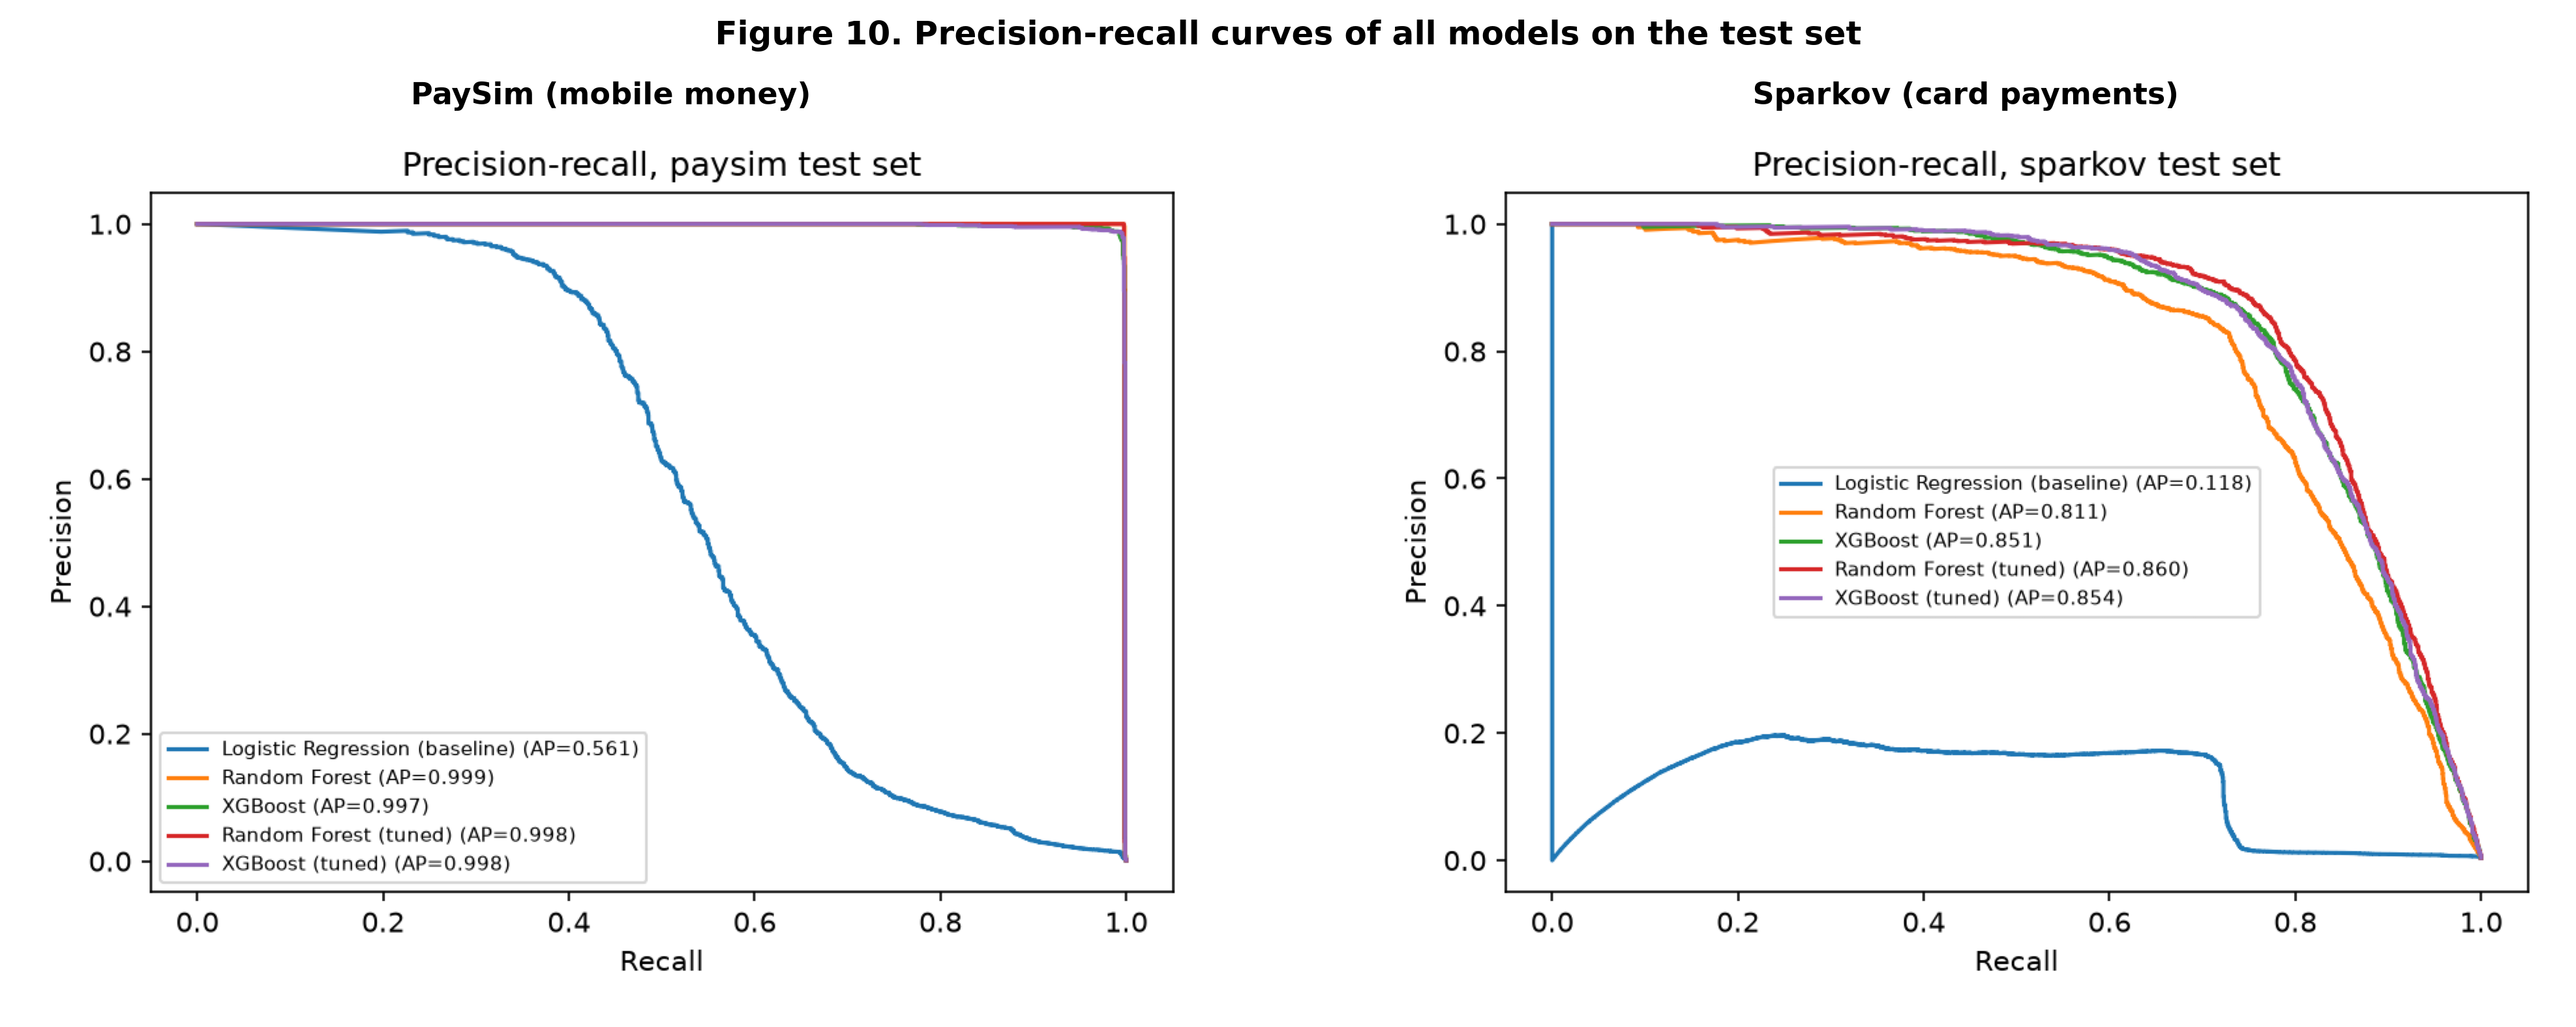
\includegraphics[width=\textwidth]{../reports/figures/fig10.png}
\caption{Precision-recall curves for the candidate models on the test sets.}
\label{fig:10}
\end{figure}

\section{Key findings}
\begin{enumerate}
  \item \textbf{PaySim:} tuned Random Forest is selected with validation PR-AUC 1.0000. On the test set it achieves PR-AUC 0.9982 and F1 0.9988, compared with PR-AUC 0.5615 and F1 0.5767 for the Logistic Regression baseline.
  \item \textbf{Sparkov:} tuned Random Forest is selected with validation PR-AUC 0.9040. On the test set it achieves PR-AUC 0.8598 and F1 0.8126, compared with PR-AUC 0.1178 and F1 0.2708 for the baseline.
  \item \textbf{Dataset-specific performance:} the selected model performs substantially better on PaySim than Sparkov. This should not be interpreted as a direct controlled comparison because the datasets, feature spaces, class distributions, and partition strategies differ.
  \item \textbf{Threshold selection matters:} a default probability threshold is not assumed to be optimal. Validation-based threshold selection is used to balance precision and recall according to F1.
  \item \textbf{Training cost:} the tuned Random Forest is the slowest final model to fit among the candidates in the recorded runs (approximately 742 seconds for PaySim and 229 seconds for Sparkov). These times are environment-dependent and exclude the separate hyperparameter search.
\end{enumerate}

% ============================================================
\chapter{Privacy, Transparency and Ethical Considerations}
\section{Privacy-conscious feature selection}
The notebook excludes direct identifiers and sensitive location/address strings from model inputs. For Sparkov, names, card numbers, street addresses, job titles, and merchant names are not used. These choices reduce the use of directly identifying attributes, but they do not by themselves guarantee anonymity or eliminate all privacy risk. Transaction data can still be sensitive and should be protected with access controls, secure storage, and retention limits in any deployment.

\section{Transparency and accountability}
Feature-importance summaries provide a global view of model reliance, but they do not explain every individual prediction. A deployed system should retain prediction scores, model versions, threshold versions, and human review outcomes where legally and operationally appropriate. High-impact actions should not rely solely on an automated flag without a suitable review and appeal process.

% ============================================================
\chapter{Challenges and Limitations}
\section{Class imbalance}
Fraud represents a small share of the records in both datasets: 0.1291\% for PaySim and 0.5789\% in the Sparkov training file. This makes accuracy a poor standalone measure. The notebook responds with class weighting or positive-class scaling and emphasizes precision-recall metrics. Nevertheless, rare-event learning remains sensitive to data quality, label noise, and changes in fraud patterns.

\section{Synthetic and historical data}
PaySim and Sparkov are distributed datasets rather than live operational feeds from the project team. Their patterns may not fully represent current real-world transaction behavior. In particular, strong performance on one dataset should not be assumed to transfer to another institution, geography, time period, or fraud strategy.

\section{Temporal and distribution shift}
The Sparkov protocol uses a later-period test file, which is a useful temporal separation, but future data can still differ from the available test period. PaySim uses stratified random splitting rather than a chronological split. For both datasets, repeated evaluation on newer data would be necessary to estimate performance under ongoing distribution drift.

\section{Threshold trade-offs}
Maximizing F1 treats precision and recall symmetrically, but a financial institution may assign different costs to false positives and false negatives. A production threshold should be selected using operational costs, review capacity, customer impact, and regulatory requirements, rather than F1 alone.

\section{Deployment scope}
The current prototype provides a FastAPI service and React dashboard around the saved model artifacts. The API validates channel-specific inputs with Pydantic schemas, computes derived PaySim balance-error features, scores transactions with the matching specialist model, and applies the threshold stored in that model's metadata. Stored scores are written to SQLite, while analytics are aggregated from the stored log rather than re-running the models. The dashboard reads analytics and model metadata, displays recent activity and model transparency information, submits manual transactions, and receives new scored records through an SSE stream. Its simulator generates illustrative records every two seconds; these are not production or user data.

The service still requires production controls such as authentication and authorization, encrypted and managed database storage, rate limiting, observability, resilient deployment, and a human investigation workflow. The current API also exposes a non-persistent \texttt{/predict} endpoint for batch scoring, with requests limited to 5,000 transactions.

% ============================================================
\chapter{Conclusion and Future Work}
\section{Conclusion}
FraudShield demonstrates a supervised-learning workflow for financial transaction fraud detection using two datasets from different payment domains. The implementation establishes Logistic Regression as a baseline and compares it with Random Forest, XGBoost, and tuned variants. Dataset-specific preprocessing and specialist models are used rather than assuming that mobile-money and card-payment records share one feature space.

The tuned Random Forest is selected for both datasets using validation PR-AUC. Its test results are strong on PaySim (F1 0.9988 and PR-AUC 0.9982) and materially improved over the baseline on Sparkov (F1 0.8126 and PR-AUC 0.8598). The trained artifacts are integrated into a functional API and dashboard that support validated scoring, SQLite-backed analytics, model transparency, and live event updates. Overall, the project meets the central technical objectives of using two datasets, preprocessing data, comparing multiple AI models, tuning models, evaluating with suitable metrics, and demonstrating an end-to-end monitoring prototype.

\section{Future improvements}
Potential next steps include:
\begin{itemize}
  \item Evaluate on additional, more recent transaction data and monitor temporal drift.
  \item Select operating thresholds using explicit financial and customer-impact costs, not F1 alone.
  \item Add calibration analysis so predicted probabilities can be interpreted more reliably.
  \item Harden the API and dashboard for deployment with authentication, authorization, rate limiting, monitoring, and secure storage.
  \item Add human review feedback and a controlled retraining process.
  \item Test ensemble strategies only if they provide measurable improvement on validation data and a final untouched test set.
\end{itemize}

% ============================================================
\chapter*{References}
\addcontentsline{toc}{chapter}{References}
\begin{enumerate}
  \item ealaxi, \textit{PaySim1: Synthetic Financial Dataset for Fraud Detection}, Kaggle. \url{https://www.kaggle.com/datasets/ealaxi/paysim1}
  \item kartik2112, \textit{Credit Card Transactions Fraud Detection Dataset}, Kaggle. \url{https://www.kaggle.com/datasets/kartik2112/fraud-detection}
  \item Scikit-learn documentation, \textit{ColumnTransformer, Pipeline, RandomizedSearchCV, and classification metrics}. \url{https://scikit-learn.org/}
  \item XGBoost documentation. \url{https://xgboost.readthedocs.io/}
  \item Supplied project implementation: \texttt{train.ipynb} and \texttt{plots.ipynb}.
  \item CT-361 Artificial Intelligence \& Expert System, Complex Computing Problem (CCP) brief, Department of Computer Science \& Information Technology.
\end{enumerate}

\end{document}